%
% Name: Accelerating Multi-dimensional Search Mid-Project Report
% Author: Donald Whyte (sc10dw@leeds.ac.uk)
%

\documentclass[notitlepage]{article}

\usepackage[margin=2.5cm]{geometry} % easy page formatting
	\geometry{letterpaper}
\usepackage{doc} %special logo commands
\usepackage{url} % formatting URLs
\usepackage{datetime} % up-to-date, automatically generated times
\usepackage{amsmath}
\usepackage{amsfonts}
\usepackage{multirow}
% For graphic files
\usepackage{graphicx}
\usepackage{epstopdf}
\DeclareGraphicsRule{.tif}{png}{.png}{`convert #1 `dirname #1`/`basename #1 .tif`.png}

\usepackage{algorithm}
\usepackage{algorithmic}

\usepackage{pdflscape}
\usepackage{rotating}
\usepackage{wrapfig}

\usepackage{cite} 

\usepackage{caption}

\usepackage{fancyhdr}
\chead{Donald Whyte}
\lhead{}
\rhead{}


\title{Accelerating Multi-dimensional Search \\ Mid-Project Report}
\author{Donald Whyte}
\date{\today}

\pagestyle{fancy} % so header appears on each page

\begin{document}

\null  % Empty line
\nointerlineskip  % No skip for prev line
\vfill
\let\snewpage \newpage
\let\newpage \relax
\maketitle
\let \newpage \snewpage
\vfill 
\break % page break

\tableofcontents

\vspace{4em}

\section{Introduction}
	\chapter{Introduction}
\label{chap:introduction}
\centerline{\rule{149mm}{.02in}}
\vspace{2cm}

\section{Problem Definition}

TODO

\section{Aims}

TODO

\section{Objectives}

TODO

\section{Minimum Requirements}

TODO

\section{Extended Requirements}

TODO

\section{Deliverables}

TODO

\section{Evaluation Criteria}

TODO

	\subsection{Aim}

This project will survey existing multi-dimensional search structures which attempt to solve the multi-dimensional search problem, identifying the major challenges of the field and how this has guided the development of structures throughout the last two decades. The core aim of the project is to implement one or more modern index structures, optimising them specifically for high-dimensional datasets. These implementation(s) will be then be evaluated with respect to their proposed performance in the literature and pre-defined baselines using test datasets. This evaluation will highlight the found performance bottlenecks in the implementations and limitations of the algorithms themselves.

	\subsection{Objectives}

The objectives of the project are:
\begin{itemize}
	\item Understand the current state and challenges of the field of multi-dimensional search
	\item Implement multi-dimensional search structures
	\item Perform performance analysis on implementations and attempt to optimise structures for greater performance on high-dimensional data
	\item Evaluate and compare performance of final structures to pre-defined baselines, unoptimised structures and their reported performance in the literature
\end{itemize}

	\subsection{Requirements}

The minimum requirements are closely related to the objectives of the project. They are:
\begin{enumerate}
	\item Produce literature review describing the current state of multi-dimensional search structures, comparing their strengths and weaknesses and highlighting core challenges of the field
	\item Implement at least one index structure and perform performance analysis of the implementation
	\item Perform one set of modifications to the implemented structure in an attempt to optimise its performance
	\item Evaluate and compare performance of final implementations to pre-defined baselines, unoptimised structures and their reported performance in the literature
\end{enumerate}

Possible extensions of the project include:
\begin{enumerate}
	\item Parallelising implementations using technologies such as Haskell, CUDA (GPGPU) or MPI
	\item Developing an entirely new index structure, which is also implemented and evaluated
\end{enumerate}

\subsection{Deliverables}

The following will be delivered upon project completion:
\begin{enumerate}
	\item Documented source code of implemented index structures
	\item User manual describing how to use the index structures
	\item Evaluation of the performance of the implemented index structures, with respect to pre-specified test data
	\item Generated synthetic data that is used for the evaluation
\end{enumerate}

\subsection{Core Assumptions}
\label{sec:core-assumptions}

Throughout the project, some assumptions have been made. These are used to narrow the scope of the project and allow more time to be spent focusing on the core aim of the project (high-dimensional data). The assumptions are:
\begin{enumerate}
	\item Datasets have a ``high" number of dimensions ($\geq 10$), meaning the performance of the index structures will be measured using data with at least 10 dimensions. However, data using a smaller number of dimensions may be used for the purposes of understanding how the implementations behave with respect to dimensionality.
	\item Datasets will be able to fit into the main memory (i.e. RAM) of the machine used for evaluation. That is, none of the data is paged to secondary memory and page accesses causing reduced performance does not need to be considered.
	\item Datasets are dynamic, meaning points may be inserted, deleted or updated at any time.
\end{enumerate}
Furthermore, the project is focused on the \textit{geometric} applications of multi-dimensional search and not databases. This is the primary reason assumption (2) has been made.

No assumptions have been made about the distribution of data. This means the implementations' performance will be evaluated using a variety of distributions.

\section{Methodology}
	This section gives information on how the project will be tackled, describing the schedule (plus any changes that have made since its initial creation), tools and technologies that will be used throughout the project.

	\subsection{Schedule}
\label{sec:schedule}

The original schedule was devised near the end of the first week of the project, on 31/01/14. The schedule was broken down into the individual tasks required to complete the defined milestones. These tasks were then grouped into different \textbf{phases}, which run sequentially (with some in parallel). The phases of the project and their milestones are:
\begin{enumerate}
	\item ``Project Definition""
	\begin{itemize}
		\item \textbf{Project Outline Defined} -- defined outline of project's aims and objects
	\end{itemize}
	\item ``Literature Review and Data Collection"
	\begin{itemize}	
		\item \textbf{Literature Review Complete} -- produced literature review of multi-dimensional search
		\item \textbf{Data Collected} --  decided and collected non-synthetic external test data sets
	\end{itemize}
	\item ``Initial Implementation"
	\begin{itemize}	
		\item \textbf{Software Deliverables Decided} -- determined index structures to implement and the technologies to use
		\item \textbf{Initial Implementation Finished} -- completed initial, unoptimised implementations of chosen index structure(s)
	\end{itemize}
	\item ``Mid-project Presentation and Report"
	\begin{itemize}	
		\item \textbf{Mid-project Presentation Delivered} -- delivered mid-project presentation to relevant research group
		\item \textbf{Mid-project Report Finished} -- submitted mid-project report
	\end{itemize}	
	\item ``Performance Tuning"
	\begin{itemize}
		\item \textbf{Software Deliverables Finished} -- produced final, optimised implementations of the index structure(s), which is ready for a final evaluation
	\end{itemize}
	\item ``Final Report Write-up"
	\begin{itemize}
		\item \textbf{Final Report Finished} -- submitted write-up of the final report
	\end{itemize}
	\item ``Student Symposium"
	\begin{itemize}
		\item \textbf{Final Presentation Delivered} -- delivered final project presentation
	\end{itemize}
\end{enumerate}

The performance tests and evaluation of the initial implementation could produce unexpected results, showing that it may be beneficial to implement an entirely different index structure or use a different technology. Therefore, deciding on a \textit{fixed} set of index structures to implement  would be unwise. Doing means there is no way to go backwards and revise the project plan if performance tests highlight a poor index structure or technology. As such, a decision has been made on a \textit{single, initial} index structure to implement. This will be evaluated and based on that evaluation, it will be optimised or it will be discarded in favour of another index structure. This will be repeated in iterations, where each iteration contains the following sub-phases:
\begin{enumerate}
	\item \textbf{Design} -- plan exactly what needs to be done in the iteration and the architectural design of the system/implementation
	\item \textbf{Build} -- implement an index structure or perform one or more optimisations
	\item \textbf{Test} -- perform correctness tests on index structure to ensure it (still) works
	\item \textbf{Performance Analysis} -- perform performance analysis on index structure developed/optimised
	\item \textbf{Evaluation} -- evaluate the produced results and use it to decide what to implement or optimise in the next iteration
\end{enumerate}
When enough iterations have passed or there is no time left to spend on the Design and Implementation phase, the iterations will stop, with the evaluation of the optimised structure(s) in last phase being the final evaluation that is used in the Final Report Write-up phase. This iterative approach is illustrated in the full project process diagram shown in Figure \ref{fig:full-project-process} in the appendix.

Figure \ref{fig:initial-schedule} and Figure \ref{fig:initial-milestone-timeline} show a Gantt chart of the phases and a timeline annotated with the project's milestones respectively. Due to the often uncertain nature of research projects, especially when one does not have much knowledge of the relevant field prior to the project, it was decided that the schedule will \textit{not} break down each phase into fine-grained sub-tasks. This is to avoid the likely situation of some of the tasks taken longer than others and having the project greatly trail away the original schedule, to the point where it's not used. Instead, these higher level phases and milestones will guide development, following the process shown in Figure \ref{fig:full-project-process}.

The plan has changed since its initial conception. The original plan stated that the initial, unoptimised implementations of the index structures should be finished before the mid-project presentation or report. The idea behind this decision was that having implementations of index structures finished before the presentation, an initial evaluation of the index structures could be performed. The results from this evaluation could then used in the presentation and report as justification for project decisions. However, due to the scope of the research field, the literature take one more week than expected. This meant that there was little time between the end of the literature review and the start of the mid-project presentation and report.

Furthermore, additional time was required to determine the nature of the data that to be used for evaluation. This knowledge informs the decisions on which index structures to implement, so it was felt that rushing into implementation may result in a poor decision on which structures to implement. Therefore, implementation has been pushed back until after the submission of the mid-project report. By doing this, there is more time to collect the research findings and make a more informed decision on the index structure to implement.

Figure \ref{fig:revised-schedule} and Figure \ref{fig:revised-milestone-timeline} show a Gantt chart of the revised phases and a timeline marked with the new milestones. The date this report has been submitted is also marked on the Gantt chart, showing what phases and milestones are left to complete before the end of the project. With the new schedule, the ``Initial Implementation" phase has been removed and the ``Performance Tuning" phase has changed to ``Design and Implementation". As a consequence, the milestones \textbf{Software Deliverables Decided} and \textbf{Initial Implementations Finished} have been removed. The \textbf{Software Deliverables Finished} milestone remains, but now marks the end of ``Design and Implementation" phase.

``Design and Implementation" encompasses the design, implementation and evaluation of the index structure. This will contain multiple iterations of the implementation process described previously. An unoptimised, functional implementation is the barest deliverable required to perform the final evaluation. To ensure this is developed, the \textbf{Initial Implementation of Software Deliverables Complete} milestone has been created. The first iteration of ``Design and Implementation" will be two weeks and will be used to develop the baselines and initial implementation of the chosen index structure. \textbf{Initial Implementation of Software Deliverables Complete} should be met at the end of this first iteration. Subsequent iterations will last a week to coincide with the weekly supervisor meetings, which will be at the start of each iteration. 

	\input{technology}
\section{Progress Report}

Referring to the schedule defined in Section \ref{sec:schedule}, as of the submission of this report, the following phases are complete: ``Project Definition", ``Literature Review and Data Collection" and ``Mid-project Presentation and Report". The following milestones have also been met: \textbf{Project Outline Defined}, \textbf{Literature Review Complete},  \textbf{Test Data Collected}, \textbf{Mid-project Presentation Delivered} and \textbf{Mid-project Report Finished}. 

This means that the project's aims, objectives and requirements have been defined, with a clear description on what the final deliverables are. Extensive research has been performed on the multi-dimensional search problem, existing solutions, their limitations and general challenges the field faces. All this information was written up into a stand-alone literature review document that has been integrated into Section \ref{sec:background-research} of this report. Which index structure to implement initially has been determined and the technologies to use to develop the implementation have also been decided. The development process has been determined which, as discussed in Section \ref{sec:schedule}, will involve multiple iterations of implementation, testing and evaluation. Finally, a presentation has been performed to the relevant research group, Computational Science and Engineering, outlining the project's aims, current progress and the design, implementation and evaluation approach which will be taken throughout the next two months.

See Section \ref{sec:next-steps} for what actions will be performed next, after the submission of this report.

\chapter{Background Research}
\label{chap:background_research}
\centerline{\rule{149mm}{.02in}}
\vspace{2cm}

\section{Literature Review}

TODO: the background research section (mostly) from mid-term report

\section{Technologies}

TODO

\section{Data for Evaluation}

TODO???

\chapter{Final Evaluation}
\label{chap:evaluation}
\centerline{\rule{149mm}{.02in}}
\vspace{2cm}

We have shown that all variations of the $kd$-tree greatly outperform the Pyramid tree for the two scientific datasets. For all synthetic data and the 3D point cloud dataset, the Pyramid tree is faster, especially with regard to point deletion.

This section will explore the reasons for this, determining which characteristics in the data cause the performance of the structures to degenerate. The section will conclude by discussing the types of data suitable for the Pyramid Tree and $kd$-Tree, along with some further discussion on the implications of the results from this evaluation.

\section{Characteristics of Test Data}

TODO

\section{Distribution of Points Across Buckets}

TODO

\section{Suitable Data for Index Structures}

TODO
\section{Next Steps: Design and Implementation}
\label{sec:next-steps}

After the submission of this report, the first iteration of the ``Design and Implementation" phase will begin. In these two weeks, the development environment will be set up and an \textbf{evaluation framework} will be created. This framework will be a C++ program that will facilate fast evaluation by allowing multiple index structures to be tested at once (using the test process described in Section \ref{sec:evaluation}), with multiple datasets. The framework will automatically generate the evaluation measures as text files and figures, so they can easily be understand and incorporated into the report. More details on the design and features of this framework will be given in the final report.

The first iteration will also implement the evaluation baselines (sequential scan and quadtree) and a chosen index structure. Initially, the Pyramid tree was going to be implemented because the structure appears to perform very well in a high-dimensional setting (based on the literature). However, through the Visualization Toolkit (VTK)\cite{vtk}, the School already has a working implementation of the Pyramid tree. Taking the School's interests into account, it was felt that implementing the Pyramid tree again, even if the new implementation has greater performance, would not provide as much insight into high-dimensional search as implementing a structure that the School does not currently have an implementation of.

Therefore, the \textbf{splay quadtree} has been chosen as the index structure to implement. It was chosen because of its self-adjusting behaviour. From the review of literature performed, it appears self-adjusting structures have not been evaluated against high-dimensional data. By implementing the splay quadtree, insight into how these types of structures perform with higher dimensions can be gained. Furthermore, the structure has low memory overhead, making it useful for storing the large astrophysics dataset described in Section \ref{sec:evaluation} whilst keeping it in main memory (see assumption (2) in Section \ref{sec:core-assumptions}). After this iteration, the remaining iterations will attempt to optimise the splay quadtree or choose to explore a different index structure if it is shown that, algorithmically, the structure performs poorly with high-dimensional data.

Additionally, the ``Final Report Write-up"" phase will begin and run in parallel with the ``Design and Implementation" phase after the first iteration.


% Include the bibliography
\bibliographystyle{unsrt}
\bibliography{refs}
\appendix
\setcounter{figure}{0} \renewcommand{\thefigure}{A.\arabic{figure}} 
\setcounter{table}{0} \renewcommand{\thetable}{A.\arabic{table}} 
\section{How Ethical Issues are Addressed}

There are no ethical issues involved with this project, as no personal data is being used in either the design, implementation or evaluation of the solution. All data used for evaluation is either synthetic data generated specifically for this project or publicly available datasets.

\section{Supplementary Material}

\begin{figure}[H]
	\centering
	\includegraphics[scale=0.6]{figures/full-project-process.pdf}
	\caption{Flow Chart of Full Project Schedule}
	\label{fig:full-project-process}
\end{figure}

\newpage

\null  % Empty line
\nointerlineskip  % No skip for prev line
\vfill
\let\snewpage \newpage
\let\newpage \relax

\begin{figure}[H]
	\centering
	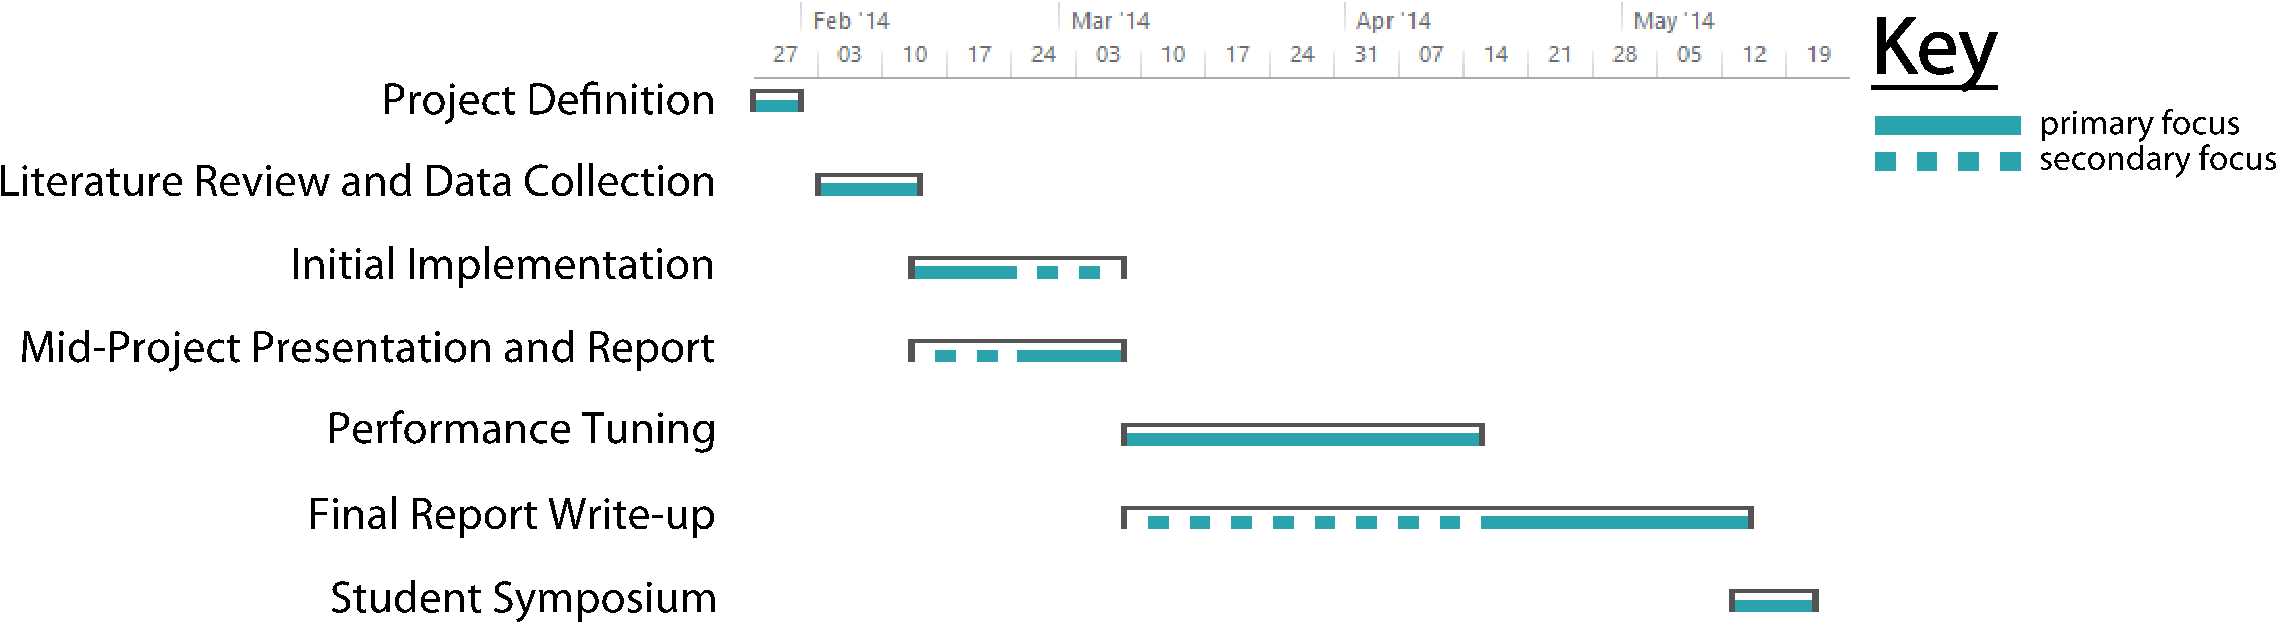
\includegraphics[scale=0.475]{figures/initial_project_schedule.pdf}
	\caption{Initial Project Schedule Created on 31/01/14. The time this report was submitted is marked on the chart to illustrate the project's current progress.}
	\label{fig:initial-schedule}
\end{figure}

\begin{figure}[H]
	\centering
	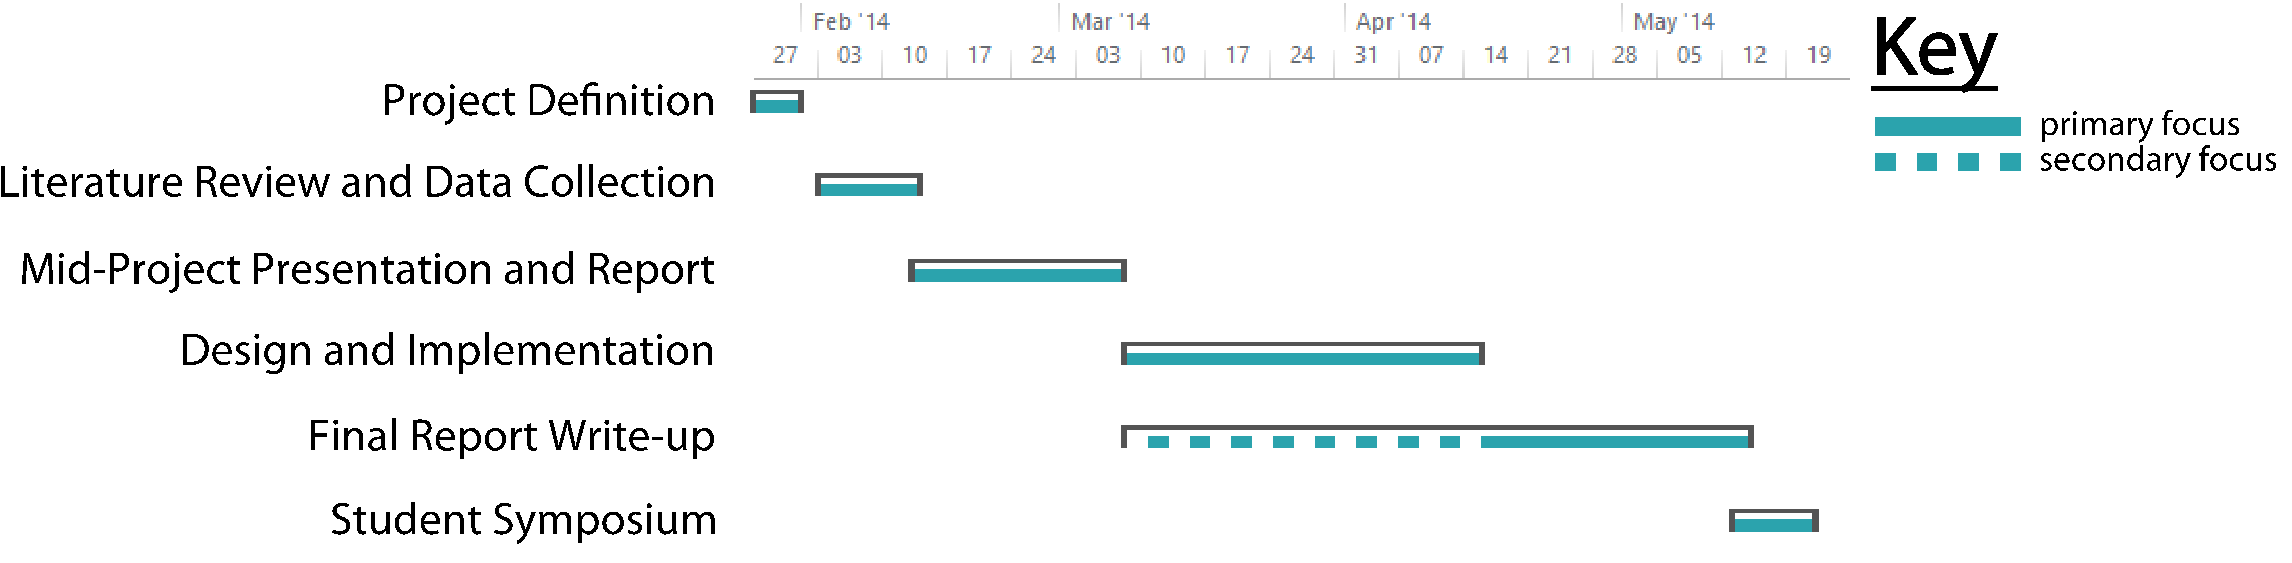
\includegraphics[scale=0.475]{figures/revised_project_schedule.pdf}
	\caption{Revised Project Schedule Created on 20/02/14. The time this report was submitted is marked on the chart to illustrate the project's current progress.}
	\label{fig:revised-schedule}
\end{figure}

\let \newpage \snewpage
\vfill 
\break % page break

\begin{landscape}	

\null  % Empty line
\nointerlineskip  % No skip for prev line
\vfill
\let\snewpage \newpage
\let\newpage \relax
	\begin{figure}[H]
		\centering
		\includegraphics[scale=0.35]{figures/md_structure_taxonomy.png}
		\caption{Multi-dimensional Search Structure Taxonomy}
		\label{fig:structure-taxonomy}
	\end{figure}
\let \newpage \snewpage
\vfill 
\break % page break

	\newpage

\null  % Empty line
\nointerlineskip  % No skip for prev line
\vfill
\let\snewpage \newpage
\let\newpage \relax
	\begin{figure}[H]
		\centering
		\centerline{ 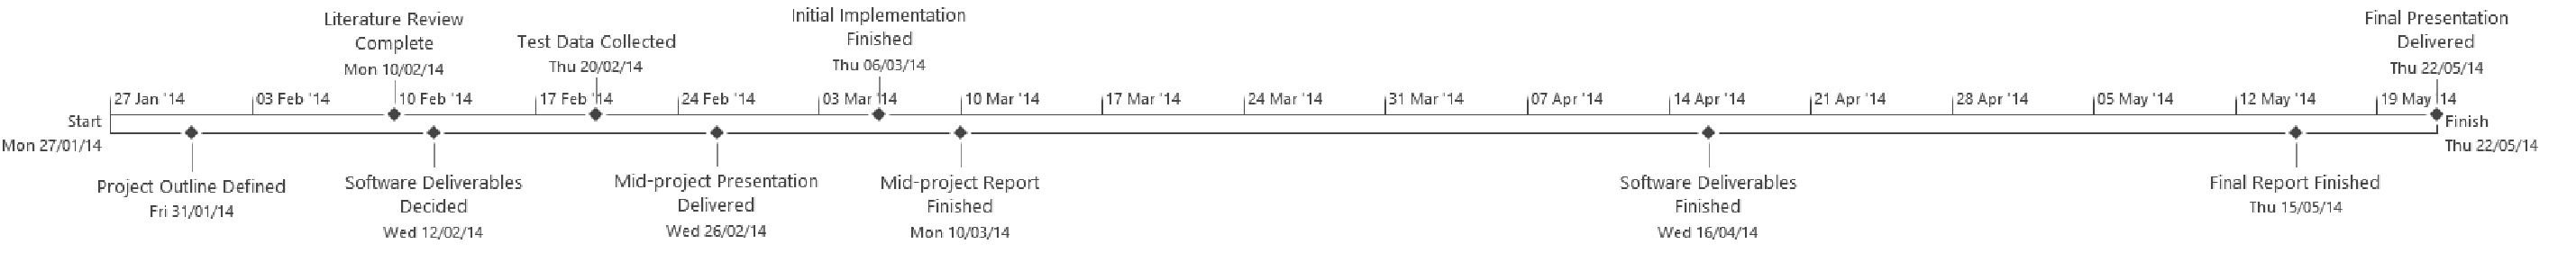
\includegraphics[scale=0.5]{figures/initial_schedule_timeline.pdf} }
		\caption{Initial Milestone Timeline Created on 20/02/14}
		\label{fig:initial-milestone-timeline}
	\end{figure}

	\begin{figure}[H]
		\centering
		\centerline{ 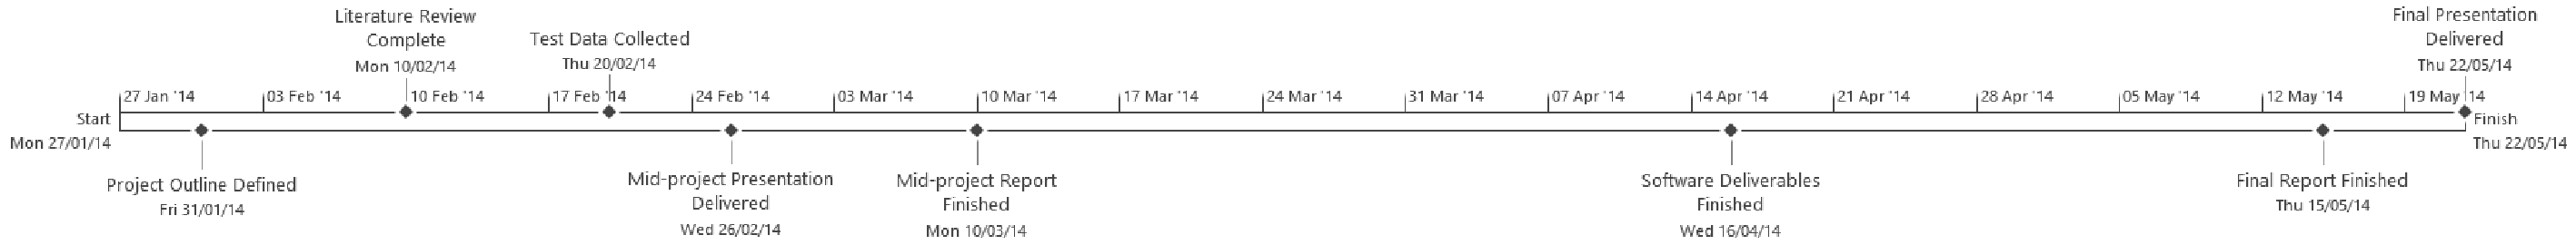
\includegraphics[scale=0.37]{figures/revised_schedule_timeline.pdf} }
		\caption{Revised Milestone Timeline Created on 20/02/14}
		\label{fig:revised-milestone-timeline}
	\end{figure}	
\let \newpage \snewpage
\vfill 
\break % page break

\end{landscape}

\begin{table}
	\centering
	\begin{tabular}{|p{2.8cm}|p{2.3cm}|p{3cm}|p{3cm}|p{3.5cm}|p{2cm}|}
		\hline
		\textbf{Index Structure} &
		\textbf{Memory Overhead} &
		\textbf{Bucket Method?} &
		\textbf{High-Dimensional Data} &
		\textbf{Complexity} \\
		\hline
		Sequential Scan & Low & No (but since data is stored contiguously, there are minimal I/O operations due to sequential access) & Often better than other structures with high $d$ (but significantly poorer performance with low $d$) & Low \\		
		B${}^{+}$-Tree & Low & Yes & One-dimensional & Low \\
		R-Tree & Moderate & Yes & Poor for $d > 10$ \cite{pyramid-tree} & Moderate \\
		Quadtree & Low with uniformly distributed data, high for skewed data due to unnecessary nodes caused by splitting sparse regions of data space & No & Poor because it tries to use balanced splits \cite{pyramid-tree} & Low \\
		Pyramid Tree & Low & Yes (based on B${}^{+}$-tree) & Good & High \\
		PK-Tree & Moderate & No (but uses similar method to reduce I/O operations) & Good & High \\
		Skip Quadtree & Moderate & No & Untested & Moderate \\
		Quadtreap & Low & No & Untested & Moderate \\
		Splay Quadtree & Moderate & No & Untested & Moderate \\
		\hline
	\end{tabular}
	\caption{Comparison of Dynamic Multi-Dimensional Structures}
	\label{tab:comparison}
\end{table}



\end{document}
